% Provenance (never printed): NSI premiere, "Representation approximative des nombres reels: notion de nombre
% flottant" (0.1 + 0.2 == 0.3 is False; consequences on equality tests). The 64-bit layout, gaps, summation order
% and special values are additions. See sources/book2/BRIEFS.md.
\chapter{Floating-Point Numbers}\label{ch:g10:floating-point}

Type \code{0.1 + 0.2 == 0.3} at Python's prompt. The answer is \code{False}. Ask for \code{0.1 + 0.2}, and Python
prints \code{0.30000000000000004}. Nothing is broken: the computer adds exactly what it was given, but it was never
given $0.1$. A memory of $64$ bits cannot hold the infinitely many digits that $0.1$ has in base $2$, so it holds
the nearest number it can.

This chapter shows which numbers a computer can store with a fractional part, how far apart they are, how the
small errors of each operation build up, and how a program should compare such numbers. Its weekend problem is a
real failure in which a tenth of a second, stored a little short, added up to a third of a second.

\begin{recall}
A number in scientific notation is written $m \times 10^{e}$ with $1 \le m < 10$, such as $6.02 \times 10^{23}$
(mathematics and physics books, grades 9 and 10). In base $2$ each position is worth twice the one on its right
(Book 1, grade 8). The previous chapter showed that a processor keeps whole numbers in a fixed number of bits;
here too the number of bits is fixed.
\end{recall}

\section{Binary fractions}\label{sec:g10:floating-point:binary-fractions}

\omcode{code/grade-10/04-floating-point/listings/point_one.py}{1}{7}{What is $0.1$, really?}%
\label{lst:g10:floating-point:point-one}

\omoutput{code/grade-10/04-floating-point/outputs/point_one.txt}{With thirty decimals, the stored \code{0.1} shows
its error; as an exact fraction, its denominator is a power of two.}\label{out:g10:floating-point:point-one}

The denominator $36{,}028{,}797{,}018{,}963{,}968$ is $2^{55}$. That is the key: the computer stores numbers whose
denominator is a power of two.

\begin{definition}[Binary fraction]\label{def:g10:floating-point:binary-fraction}
A \emph{binary fraction}\index{binary fraction} is a number written in base $2$ with digits after a binary point:
$0.b_1 b_2 b_3 \dots$ stands for $b_1 \cdot \tfrac12 + b_2 \cdot \tfrac14 + b_3 \cdot \tfrac18 + \dots$, each
position worth half of the one on its left. A number has a binary fraction with finitely many digits exactly when
it is a fraction whose denominator can be a power of two.
\end{definition}

For example, $0.375 = \tfrac38 = \tfrac14 + \tfrac18$ is $0.011$ in base $2$. But $\tfrac1{10}$ cannot be written
with a power of two as denominator ($10$ has the factor $5$), so its binary digits never end. They are found by
\emph{doubling}: multiply by $2$; the whole part ($0$ or $1$) is the next digit; keep the fractional part and repeat.

\begin{omfigure}
\begin{tikzpicture}[font=\small]
  \matrix[matrix of nodes, nodes={minimum height=5.5mm, anchor=center, inner sep=2pt},
    column 1/.style={nodes={minimum width=16mm}}, column 2/.style={nodes={minimum width=20mm}},
    column 3/.style={nodes={minimum width=14mm, font=\small\bfseries}},
    row 1/.style={nodes={font=\footnotesize\itshape}}] (m) {
    fraction & doubled & digit \\
    $0.1$ & $0.2$ & 0 \\
    $0.2$ & $0.4$ & 0 \\
    $0.4$ & $0.8$ & 0 \\
    $0.8$ & $1.6$ & 1 \\
    $0.6$ & $1.2$ & 1 \\
    $0.2$ & $0.4$ & 0 \\
    $0.4$ & $0.8$ & 0 \\
    $\vdots$ & & \\
  };
  \draw (m-1-1.south west) -- (m-1-3.south east);
  \draw[omProp, thick, rounded corners] (m-3-1.north west) rectangle (m-6-3.south east);
  \draw[ptr, omProp] ([xshift=2mm]m-7-3.east) to[bend right=35] node[right, align=left, font=\footnotesize]
    {$0.2$ again: the four digits\\$0011$ repeat for ever} ([xshift=2mm]m-3-3.east);
\end{tikzpicture}

{\small The doubling method on $0.1$. The fraction $0.2$ comes back after four steps, so $0.1$ is
$0.0\,0011\,0011\,0011\dots$ in base $2$.}
\end{omfigure}

\omcode{code/grade-10/04-floating-point/listings/to_binary_fraction.py}{1}{19}{The doubling method, computed exactly
with fractions.}\label{lst:g10:floating-point:to-binary-fraction}

\omoutput{code/grade-10/04-floating-point/outputs/to_binary_fraction.txt}{$0.375$ ends after three digits; $0.1$ and
$\tfrac13$ never end.}\label{out:g10:floating-point:to-binary-fraction}

A computer that keeps a fixed number of binary digits must therefore cut $0.1$ somewhere. Whatever it keeps is
slightly more or slightly less than $0.1$; the decimal number that we type is not the number it stores.

\section{Sign, exponent and significand}\label{sec:g10:floating-point:format}

Keeping a fixed number of digits \emph{after the point} would waste them: a distance in kilometres between stars
and the size of an atom in metres need digits in very different places. Scientific notation solves this by letting
the point float, and computers do the same in base $2$.

\begin{definition}[Floating-point number]\label{def:g10:floating-point:float}
A \emph{floating-point number}\index{floating-point number} is a number written $\pm m \times 2^{e}$, where the
\emph{sign}\index{sign (floating-point)} is $+$ or $-$, the \emph{exponent}\index{exponent (floating-point)} $e$ is a
whole number, and the \emph{significand}\index{significand} $m$ is a \omterm{def:g10:floating-point:binary-fraction}{binary fraction} with $1 \le m < 2$ and a fixed
number of digits. Each of the three parts is stored in a fixed number of bits.
\end{definition}

% ledger: g10:binary64-53
Python's \code{float} is the $64$-bit format of the IEEE 754 standard, used by almost every computer. Its bits are
split $1 + 11 + 52$: one bit for the \omterm{def:g10:floating-point:float}{sign}; eleven bits for the \omterm{def:g10:floating-point:float}{exponent}, stored with $1023$ added so that it is never
negative; and fifty-two bits for the digits of the \omterm{def:g10:floating-point:float}{significand} after its point. The digit before the point is always
$1$, so it is not stored: the \omterm{def:g10:floating-point:float}{significand} has $53$ significant bits.

\begin{omfigure}
\begin{bytefield}[bitwidth=0.24cm, bitheight=6ex]{64}
  \bitheader[endianness=big]{0,52,63} \\
  \bitbox{1}{\tiny 0} & \bitbox{11}{\scriptsize\ttfamily 01111111011} &
  \bitbox{52}{\scriptsize\ttfamily 1001100110011001100110011001100110011001100110011010}
\end{bytefield}

\smallskip
{\small The $64$ bits of the stored \code{0.1}: \omterm{def:g10:floating-point:float}{sign} $0$; \omterm{def:g10:floating-point:float}{exponent} field $1019$, that is $e = 1019 - 1023 = -4$;
fraction bits $1001\,1001 \dots 1010$. The value is $1.1001\,1001\dots1010 \times 2^{-4}$ in base $2$. The last digits
$\dots 1010$ instead of $\dots 1001\,1001$ show that the digits were rounded up.}
\end{omfigure}

The module \code{struct} turns a float into its eight bytes, which the listing below cuts into the three fields.

\omcode{code/grade-10/04-floating-point/listings/float_bits.py}{1}{18}{The three fields of a 64-bit
float.}\label{lst:g10:floating-point:float-bits}

\omoutput{code/grade-10/04-floating-point/outputs/float_bits.txt}{$1.0$ is $1 \times 2^0$ and $-2.5$ is
$-1.01 \times 2^1$ in base $2$. \code{float.hex} writes the \omterm{def:g10:floating-point:float}{significand} in hexadecimal; the last line prints the
number of significant bits, the largest \omterm{def:g10:floating-point:float}{exponent} and the largest float.}\label{out:g10:floating-point:float-bits}

Sixty-four bits are too many to work by hand. A toy format of $8$ bits has the same structure: one \omterm{def:g10:floating-point:float}{sign} bit,
$3$ \omterm{def:g10:floating-point:float}{exponent} bits $E$ stored with $3$ added, and $4$ fraction bits $F$; a positive pattern stands for
$(1 + F/16) \times 2^{E - 3}$. (The toy format has no zero and no \omterm{def:g10:floating-point:special}{special values}; the real one reserves some
patterns for them.)

\omcode{code/grade-10/04-floating-point/listings/toy_float.py}{1}{15}{Every value of the toy
format.}\label{lst:g10:floating-point:toy-float}

\omoutput{code/grade-10/04-floating-point/outputs/toy_float.txt}{Sixteen values for each \omterm{def:g10:floating-point:float}{exponent}, evenly spaced
inside the group; the gap doubles from one group to the next.}\label{out:g10:floating-point:toy-float}

\begin{omfigure}
\begin{tikzpicture}
  \begin{axis}[omrecord, width=\linewidth, height=3.6cm, xmin=0, xmax=32, ymin=-0.6, ymax=0.9,
      ytick=\empty, axis y line=none, xtick={0,1,2,4,8,16,31}, xlabel={value}, grid=none,
      point meta=explicit, colormap={om}{color=(omDef) color=(omProp)}]
    \addplot[only marks, mark=|, mark size=4pt, scatter, scatter src=explicit]
      table[x=value, y expr=0, meta=exponent] {code/grade-10/04-floating-point/figures/toy_float_points.dat};
    \node[font=\footnotesize, anchor=south west] at (axis cs:0,0.35) {crowded near $0$};
    \node[font=\footnotesize, anchor=south] at (axis cs:24,0.35) {gap $1$ between $16$ and $31$};
  \end{axis}
\end{tikzpicture}

{\small The $128$ values of the toy format on a number line. There are as many values between $16$ and $31$ as
between $\tfrac18$ and $\tfrac14$: \omterm{def:g10:floating-point:float}{floating-point numbers} keep the same number of significant digits, not the same
number of digits after the point.}
\end{omfigure}

\section{Gaps between neighbours}\label{sec:g10:floating-point:gaps}

The same happens in the 64-bit format. Between $1$ and $2$ the \omterm{def:g10:floating-point:float}{significands} $1.00\dots0$ to $1.11\dots1$ give
$2^{52}$ values, evenly spaced by $2^{-52}$; between $2$ and $4$, the same number of values spaced by $2^{-51}$; and so
on. \code{math.nextafter(x, math.inf)} gives the next float above \code{x}, and \code{math.ulp(x)} the gap.

\begin{omfigure}
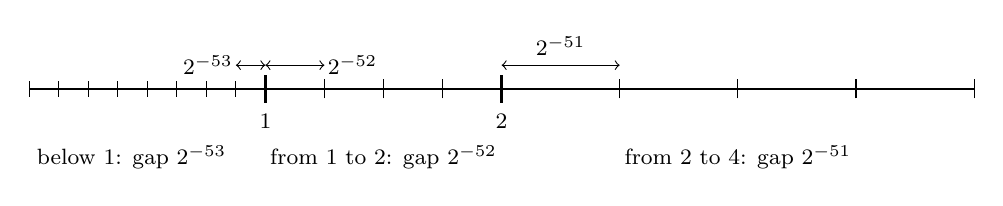
\begin{tikzpicture}[font=\footnotesize]
  \draw[thick] (0,0) -- (12,0);
  \foreach \i in {0,...,7} \draw (0.375*\i,-0.1) -- (0.375*\i,0.1);
  \foreach \i in {0,...,3} \draw (3+0.75*\i,-0.12) -- (3+0.75*\i,0.12);
  \foreach \i in {0,...,4} \draw (6+1.5*\i,-0.12) -- (6+1.5*\i,0.12);
  \draw[very thick] (3,-0.18) -- (3,0.18) (6,-0.18) -- (6,0.18);
  \node[below=2mm] at (3,0) {$1$};
  \node[below=2mm] at (6,0) {$2$};
  \draw[<->] (2.625,0.3) -- (3,0.3) node[pos=0, left, inner sep=1pt] {$2^{-53}$};
  \draw[<->] (3,0.3) -- (3.75,0.3) node[pos=1, right, inner sep=1pt] {$2^{-52}$};
  \draw[<->] (6,0.3) -- node[above] {$2^{-51}$} (7.5,0.3);
  \node[below=6mm, align=center] at (1.3,0) {below $1$: gap $2^{-53}$};
  \node[below=6mm, align=center] at (4.5,0) {from $1$ to $2$: gap $2^{-52}$};
  \node[below=6mm, align=center] at (9,0) {from $2$ to $4$: gap $2^{-51}$};
\end{tikzpicture}

{\small Neighbouring floats around $1$ and $2$, far from scale: the ticks stand for floats. The gap doubles at
each power of two.}
\end{omfigure}

\omcode{code/grade-10/04-floating-point/listings/gaps.py}{1}{7}{Next floats and gaps.}%
\label{lst:g10:floating-point:gaps}

\omoutput{code/grade-10/04-floating-point/outputs/gaps.txt}{From $2^{52}$ on the gap is $1$; from $2^{53}$ on it is
$2$, and $2^{53} + 1$ is not a float.}\label{out:g10:floating-point:gaps}

\begin{definition}[Machine epsilon]\label{def:g10:floating-point:epsilon}
The \emph{machine epsilon}\index{machine epsilon} of a floating-point format is the gap between $1$ and the next
number of the format. For the 64-bit format it is $2^{-52} \approx 2.2 \times 10^{-16}$.
\end{definition}

\begin{proposition}[Relative size of the gaps]\label{prop:g10:floating-point:relative-gap}
For a 64-bit float $x$ with $2^{e} \le x < 2^{e+1}$, the gap to the next float is $2^{e-52}$, which lies between
$\tfrac12 \varepsilon x$ and $\varepsilon x$, where $\varepsilon = 2^{-52}$. All whole numbers from $0$ to $2^{53}$ are
floats, but $2^{53} + 1$ is not.
\end{proposition}

\begin{proof}
On $[2^e, 2^{e+1})$ the floats are $m \times 2^e$ with $m = 1 + k/2^{52}$ for $k = 0, \dots, 2^{52} - 1$: the gap is
$2^{e} \times 2^{-52}$. Since $2^e \le x < 2^{e+1}$, that gap is between $\tfrac12 \varepsilon x$ and $\varepsilon x$.
For $e \le 52$ the gap is at most $1$, so every whole number below $2^{53}$ is a float; for $e = 53$ the gap is $2$,
so after $2^{53}$ the next float is $2^{53} + 2$.
\end{proof}

So a float has about $16$ significant decimal digits, whatever its size. That is plenty for most measurements; the
trouble comes when errors build up.

\section{Rounding error and how it builds up}\label{sec:g10:floating-point:rounding}

\begin{definition}[Rounding error]\label{def:g10:floating-point:rounding-error}
When the exact result of an operation, or a number typed in decimal, is not a float, the computer keeps the nearest
float. The difference between the exact value and the stored value is the \emph{rounding
error}\index{rounding error}. For one operation it is at most half the gap, that is, at most $\tfrac12\varepsilon$
times the size of the result.
\end{definition}

One \omterm{def:g10:floating-point:rounding-error}{rounding error} is tiny. But each addition makes a new one, and a program that adds many numbers adds their
errors too.

\omcode{code/grade-10/04-floating-point/listings/sum_tenths.py}{1}{10}{Adding tenths, by a loop and with
\code{math.fsum}.}\label{lst:g10:floating-point:sum-tenths}

\omoutput{code/grade-10/04-floating-point/outputs/sum_tenths.txt}{A million additions lose about $1.3 \times 10^{-6}$.
The last line adds the same three numbers in two orders.}\label{out:g10:floating-point:sum-tenths}

% ledger: g10:py-fsum
The function \code{math.fsum} keeps track of the digits lost at each step and rounds only once, at the end; it is
slower, and exact enough to give $1.0$ and $100000.0$. The last line shows that the order of the additions matters:
$10^{16} + 1$ is not a float (it lies above $2^{53}$, where the gap is $2$), so the $1$ is lost if it is added to
$10^{16}$ first, and kept if $10^{16} - 10^{16}$ is computed first. Addition of floats is not associative.

The worst case is the subtraction of two nearly equal numbers. Their leading digits cancel, and what remains is
mostly the \omterm{def:g10:floating-point:rounding-error}{rounding error} they carried.

\omcode{code/grade-10/04-floating-point/listings/cancel.py}{1}{6}{Three ways to compute $1 - \cos x$ for a small
$x$.}\label{lst:g10:floating-point:cancel}

\omoutput{code/grade-10/04-floating-point/outputs/cancel.txt}{The direct formula gives $0$: every correct digit was
lost.}\label{out:g10:floating-point:cancel}

For $x = 10^{-8}$, $\cos x$ is so close to $1$ that it rounds to exactly $1.0$, and the subtraction gives $0$. The
formula $1 - \cos x = 2\sin^2(x/2)$, from trigonometry, avoids the subtraction and gives the right value,
$5 \times 10^{-17}$, very nearly $x^2/2$.

\begin{method}[Keeping rounding errors small]\label{met:g10:floating-point:keep-small}
\begin{enumerate}
  \item Count with whole numbers when you can: money in cents, time in ticks, and compute the decimal value only to
    print it.
  \item Compute a value directly (\code{k * 0.1}) rather than by adding a step many times.
  \item Avoid subtracting nearly equal numbers; look for a formula that does not.
  \item To add many numbers, use \code{math.fsum}.
\end{enumerate}
\end{method}

\section{Comparing floats, and special values}\label{sec:g10:floating-point:compare}

Since computed floats carry \omterm{def:g10:floating-point:rounding-error}{rounding errors}, \code{==} between two of them asks the wrong question. The right
question is whether they are close.

\begin{method}[Comparing two floats]\label{met:g10:floating-point:isclose}
Use \code{math.isclose(a, b)}, which is true when $|a - b| \le 10^{-9} \times \max(|a|, |b|)$: a \emph{relative}
tolerance, which scales with the numbers. Near zero a relative tolerance is too strict (only $0$ is close to $0$), so
add an \emph{absolute} tolerance chosen from the problem: \code{math.isclose(a, b, abs_tol=1e-9)}.
\end{method}

The format also reserves some patterns for results that are not ordinary numbers.

\begin{definition}[Special values]\label{def:g10:floating-point:special}
The \emph{special values}\index{special values (infinity, NaN)} of the floating-point format are \code{inf} and
\code{-inf}, the results of an overflow beyond the largest float; \code{nan} (``not a number''), the result of an
operation that has no meaning, such as $\infty - \infty$; and \code{-0.0}, a zero that remembers it came from the
negative side. Every comparison with \code{nan} is false, even \code{nan == nan}.
\end{definition}

\omcode{code/grade-10/04-floating-point/listings/compare.py}{1}{11}{Closeness and \omterm{def:g10:floating-point:special}{special
values}.}\label{lst:g10:floating-point:compare}

\omoutput{code/grade-10/04-floating-point/outputs/compare.txt}{\code{max} gives a different answer depending on
where the \code{nan} is.}\label{out:g10:floating-point:compare}

The fourth line shows why \code{nan} is dangerous: \code{max(nan, 1.0)} keeps \code{nan} because \code{1.0 > nan} is
false, while \code{max(1.0, nan)} keeps \code{1.0} for the same reason. A missing measurement stored as \code{nan}
can silently change a result. Test for it with \code{math.isnan}, never with \code{==}.

\begin{history}[A standard for floating-point arithmetic]
% ledger: g10:ieee754-1985, g10:ieee754-2019
Before the 1980s, each make of computer had its own floating-point format and its own rounding, and the same
program could give different answers on two machines. The IEEE published a common standard, IEEE 754, in 1985; its
current edition dates from 2019. Thanks to it, the results of this chapter's listings are the same on every computer
that runs Python.
\end{history}

\section{Exercises}\label{sec:g10:floating-point:exercises}

\begin{exercise}[$\star$]\label{exo:g10:floating-point:1}
What do \code{0.1 * 3}, \code{0.1 * 3 == 0.3}, \code{0.5 * 3 == 1.5} and \code{0.25 + 0.5 == 0.75} print? Why are
the last two \code{True}?
\end{exercise}

\begin{exercise}[$\star$]\label{exo:g10:floating-point:2}
Write $0.375$, $0.8125$ and $5.75$ in base $2$, by the doubling method for the fractional parts.
\end{exercise}

\begin{exercise}[$\star$]\label{exo:g10:floating-point:3}
Find the binary digits of $\tfrac13$ by the doubling method, and show that they repeat. What is the period?
\end{exercise}

\begin{exercise}[$\star$]\label{exo:g10:floating-point:4}
What do \code{math.isclose(1.0, 1.0 + 1e-10)}, \code{math.isclose(1e-10, 2e-10)} and
\code{math.isclose(1e-10, 2e-10, abs_tol=1e-9)} return? Explain each with the formula of the method.
\end{exercise}

\begin{exercise}[$\star$]\label{exo:g10:floating-point:5}
The loop \code{x = 0.0} then \code{while x != 1.0: x = x + 0.1} never stops. Using the output on adding tenths, say
why, and rewrite the loop so that it stops after ten turns.
\end{exercise}

\begin{exercise}[$\star\star$]\label{exo:g10:floating-point:6}
A 64-bit float has the \omterm{def:g10:floating-point:float}{sign} bit $1$, the \omterm{def:g10:floating-point:float}{exponent} field \code{10000000010} and the fraction bits \code{1100} followed by
$48$ zeros. What number is it?
\end{exercise}

\begin{exercise}[$\star\star$]\label{exo:g10:floating-point:7}
Every float is a fraction with a power of two as denominator, so its binary digits end. Write
\code{exact_binary(x)}, which returns all the binary digits after the point of a float $0 \le x < 1$, using
\code{Fraction(x)} and the doubling method. How many digits does the stored \code{0.1} have?
\end{exercise}

\begin{exercise}[$\star\star$]\label{exo:g10:floating-point:8}
What is the gap between $2^{20}$ and the next float? How many floats are there between $2^{20}$ and $2^{21}$? Check
with \code{math.ulp}.
\end{exercise}

\begin{exercise}[$\star\star$]\label{exo:g10:floating-point:9}
What do \code{(1e16 + 1.0) + 1.0}, \code{1e16 + (1.0 + 1.0)} and \code{sum([1e16, 1.0, 1.0])} print? Which order of
addition keeps the most digits?
\end{exercise}

\begin{exercise}[$\star\star$]\label{exo:g10:floating-point:10}
A timer fires every $0.1$ s, and a program computes the time of the $k$th firing either with \code{t += 0.1} or as
\code{k * 0.1}. For the first $30$ firings, which method gives \code{k / 10} exactly more often? Explain with the
method of this chapter.
\end{exercise}

\begin{exercise}[$\star\star$]\label{exo:g10:floating-point:11}
Write \code{almost_equal(a, b, rel, abs_)} that combines a relative and an absolute tolerance as
\code{math.isclose} does, and test it against \code{math.isclose} on random pairs.
\end{exercise}

\begin{exercise}[$\star\star\star$]\label{exo:g10:floating-point:12}
Prove that $2^{53} + 1$ is not a 64-bit float, and that $2^{53} + 2$ is. What does \code{2**53 + 1.0} give?
\end{exercise}

\begin{exercise}[$\star\star\star$]\label{exo:g10:floating-point:13}
In the toy format, how many values lie in $[1, 2)$, in $[2, 4)$, and in all? Which whole numbers from $1$ to $31$ are
values of the format? Which is the smallest whole number that is not?
\end{exercise}

\begin{exercise}[$\star\star\star$]\label{exo:g10:floating-point:14}
The roots of $x^2 + bx + c$, for $b > 0$ large and $c = 1$, are found with the formula
$\left(-b \pm \sqrt{b^2 - 4c}\right)/2$. For $b = 10^8$, compute the small root with the $+$ \omterm{def:g10:floating-point:float}{sign}, then as
$c$ divided by the large root (the product of the roots is $c$). Explain the difference, and say which is right.
\end{exercise}

\begin{exercise}[$\star\star\star$]\label{exo:g10:floating-point:15}
A weather station's readings are floats, and a missing reading is stored as \code{nan}. The function
\code{largest} starts with \code{best = readings[0]} and keeps any \code{r > best}. What does it return for
\code{[nan, 3.0, 7.0]}, and for \code{[3.0, nan, 7.0]}? Correct it.
\end{exercise}

\section{Problem: A Clock That Drifts}\label{sec:g10:floating-point:problem}

\begin{problem}[{Weekend problem --- a third of a second in a hundred hours}]\label{pb:g10:floating-point:1}
% ledger: g10:patriot-date, g10:patriot-deaths, g10:patriot-24bit, g10:patriot-100h, g10:patriot-100h-shift, g10:patriot-8h
On 25~February 1991, an air-defence system at Dhahran, in Saudi Arabia, failed to intercept an incoming missile,
which hit a barracks and killed $28$ soldiers. A report of the U.S. General Accounting Office found the cause: the
system counted time in tenths of a second as a whole number, and converted it to seconds with registers only $24$
bits long; the conversion lost precision, and the error grew the longer the system ran. The battery had been
running for about $100$ hours. The report's table gives the error: $0.0275$~s after $8$ hours, $0.3433$~s after
$100$ hours, and a shift of $687$~m in where the system looked for its target. This problem rebuilds the table; the
program \code{exercises/clock_drift.py} does the exact arithmetic.

\medskip\noindent\textbf{Part I --- A tenth, chopped.}
\begin{enumerate}
  \item Using the figure on the doubling method, write the first $27$ binary digits of $0.1$ after the point.
  \item A value is \emph{chopped} after $p$ binary places when the digits after the $p$th are dropped. Write the
    function \code{chopped(x, bits)} of the program in words.
  \item Show that the digits of $0.1$ dropped after the $23$rd place are $0.11001100\dots$ times $2^{-23}$, that
    is $0.8 \times 2^{-23}$.
  \item Deduce the error of one tenth chopped after $23$ places, and give it in seconds to three significant digits.
\end{enumerate}

\medskip\noindent\textbf{Part II --- The error per tick.}
\begin{enumerate}[resume]
  \item The clock adds the chopped tenth at each tick. How many ticks are there in one hour?
  \item Compute the drift after one hour, and compare it with the report's $0.0034$~s.
  \item In the same way, compute the drift after $8$ hours and compare it with $0.0275$~s.
  \item Why does the drift grow in proportion to the running time?
\end{enumerate}

\medskip\noindent\textbf{Part III --- A hundred hours.}
\begin{enumerate}[resume]
  \item How many ticks are there in $100$ hours?
  \item Compute the drift after $100$ hours from the error per tick.
  \item Run the program and compare its six lines with the report's values at $1$, $8$, $20$, $48$, $72$ and $100$
    hours.
  \item The program also computes the drift for a tenth chopped after $24$ places. What is it after $100$ hours?
    Which of the two matches the report?
  \item Rebooting the system resets the count of ticks to $0$. What drift would remain if it were rebooted every $8$
    hours?
\end{enumerate}

\medskip\noindent\textbf{Part IV --- From time to distance.}
\begin{enumerate}[resume]
  \item An error in time becomes an error in position: an object moving at $v$ metres per second covers $v \times t$
    metres in $t$ seconds. From the report's $0.3433$~s and $687$~m, find the speed it assumed, to the nearest
    $10$~m/s.
  \item With that speed, check the report's shift of $55$~m after $8$ hours.
  \item How far would the target have moved during the drift after $100$ hours with the $24$-place tenth?
  \item The error could have been avoided by counting time only in whole ticks. Explain how, using the method on
    keeping \omterm{def:g10:floating-point:rounding-error}{rounding errors} small.
  \item Suppose instead that the time is computed as the number of ticks times a 64-bit \code{0.1}, whose \omterm{def:g10:floating-point:rounding-error}{rounding
    error} is about $5.6 \times 10^{-18}$, with one more rounding for the product. Estimate the error after $100$
    hours. Is it zero?
  \item State the result: the error of one tick, and the drift after $100$ hours, computed exactly, compared with the
    report.
\end{enumerate}
\end{problem}
